\capitulo{6}{Trabajos relacionados}\label{cap:TrabRel}
El progreso de la calidad de vida de pacientes con la enfermedad de \textit{Parkinson} mejora con el paso del tiempo y eso es debido a las múltiples investigaciones que se hacen sobre ello. Un ámbito en el que es fundamental avanzar es en la creación de sistemas de rehabilitación \textit{online}. 

La creación de sistemas que por medio de la visión artificial puedan evaluar ejercicios de un paciente, hace que tanto los pacientes como el terapeuta reciban una retroalimentación inmediata y precisa de los ejercicios que se realizan. 

A continuación se van a exponer algunas de las investigaciones que van aportando nuevos conocimientos en la mejora de las técnicas existentes. 

\subsection{Feasibility of Using Dynamic Time Warping to Measure Motor States in Parkinson’s Disease ~\cite{aghanavesi2020feasibility}} 

En este artículo publicado por las universidades de Dalarna y Halmstad, ambas en Suiza, estudia la viabilidad de aplicar \textbf{DTW} para el análisis de los estados motores en pacientes con la enfermedad de \textit{Parkinson}. Para ello se implantó un dispositivo en el tobillo de cada uno de los 19 pacientes que participaron en el proceso.

Este estudio persigue evaluar los síntomas motores de los pacientes, y como los mismos suelen sufrir caídas, está sobretodo enfocado a detectar los movimientos de las extremidades inferiores del cuerpo humano. Los datos fueron extraídos de diferentes señales de golpeo del pie que ejercían los pacientes sobre el suelo, en concreto se almacenaban seis señales por cada golpeo. 

El conjunto de datos fue creado a partir de las seis señales, $X_{acc}$, $Y_{acc}$, $Z_{acc}$ representan la aceleración de golpeo del pie, y $X_{gyr}$, $Y_{gyr}$, $Z_{gyr}$ para representar el giroscopio. Las medidas de distancia fueron calculadas cada dos pruebas consecutivas, como se puede observar en la figura \ref{f:datosdds} y se construyó una puntuación de distancia del estado motor, DDS.

\begin{figure}
 \centering
    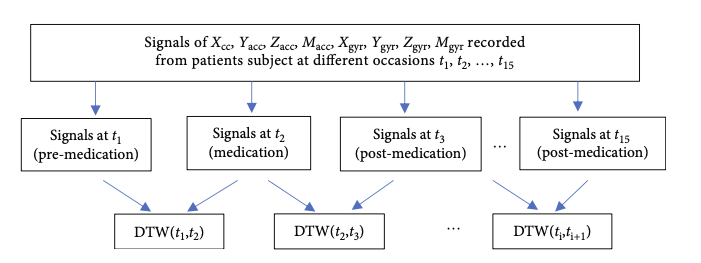
\includegraphics[width=\textwidth]{plantillaLatex-master/img/DTW_xyz.png}
    \caption{Arquitectura del conjunto de datos.}
    \label{f:datosdds}
\end{figure}


Una serie de especialistas en trastornos del movimiento clasificaron los estados motores de los pacientes de acuerdo a la TRS, \textit{Escala de Respuesta al Tratamiento}. Con los datos generados por pacientes que sufrían la enfermedad de \textit{Parkinson} se pudo concluir que el DDS medio fue capaz de identificar entre pacientes con EP en estado avanzado y clasificar los cambios del estado motor con buena precisión. 

Por último se identificaron características basadas en DTW para cada paciente, por lo que se puede concluir que por medio de esta disciplina se puede proporcionar información sobre el estado motor de los pacientes con EP avanzada. 


\subsection{A Dynamic Time Warping Based Algorithm to Evaluate Kinect-Enabled Home-Based Physical Rehabilitation Exercises for Older People ~\cite{s19132882}} \label{cap:TrabRelTaiChi}

En este artículo redactado por el Departamento de Ingeniería Industrial y de Sistemas del  Instituto Avanzado de Ciencia y Tecnología de Corea, se puede observar el uso de técnicas de visión por computador para calcular características sobre las posicione humanas en distintos instantes de tiempo. 

A través de la tecnología \texttt{\textit{Kinect}} \footnote{\textit{Kinect} es un sistema desarrollado por Microsoft que permite reconocer la figura de un individuo en 3D a partir de una cámara RGBD} el movimiento humano es almacenado en forma de coordenadas. Estas coordenadas serán analizadas para determinar una similitud entre el movimiento del entrenador y el movimiento del usuario final. En la figura \ref{f:KinectSkeleton} se puede observar como se representarían los esqueletos obtenidos mediante esta técnica


\begin{figure}
 \centering
    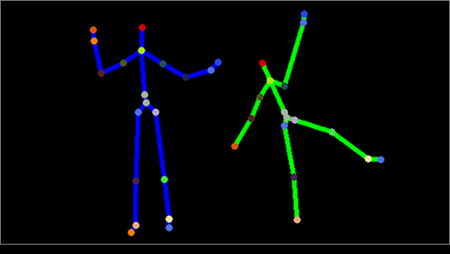
\includegraphics[width=0.6\textwidth]{plantillaLatex-master/img/KinectSkeleton.png}
    \caption{Obtención del esqueleto mediante la tecnología \textit{Kinect}.}
    \label{f:KinectSkeleton}
\end{figure}


De los esqueletos anteriores, para la comparación de posiciones solo se usan las relativas a las extremidades superiores e inferiores. El primer paso que toma el algoritmo es cuantificar la diferencia entre cada una de estas poses del entrenador con las del usuario final. En la figura \ref{f:KinectSkeleton2} se puede comprender como a través de la ley del coseno se puede calcular la diferencia entre la posición del entrenador y del aprendiz. 

\begin{figure}[H]
 \centering
    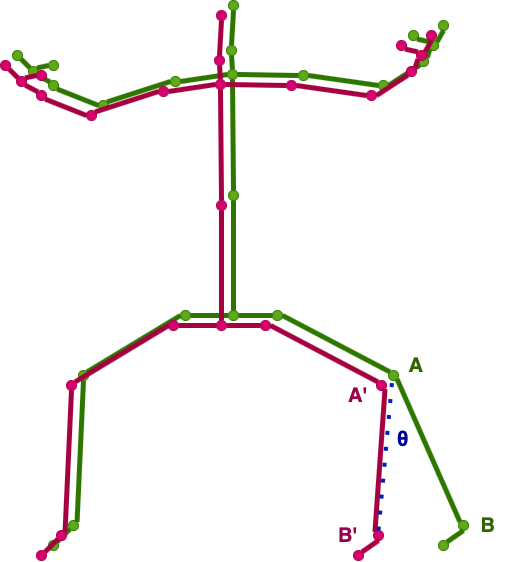
\includegraphics[width=0.4\textwidth]{plantillaLatex-master/img/KinectSkeleton2.png}
    \caption{Diferencia de posiciones en esqueletos.}
    \label{f:KinectSkeleton2}
\end{figure}


La comparación de movimientos se realiza, una vez localizadas las dos secuencias a comparar, se aplica \emph{DTW} para determinar la coincidencia óptima. Se obtendrían dos matrices de ocho filas y \textit{n} columnas, siendo \textit{n} el número de movimientos realizados por el individuo y ocho las posiciones óseas correspondientes a las extremidades superiores e inferiores. Además se tuvo en cuenta la orientación del individuo.

Los resultados obtenidos en este estudio son una puntuación de rendimiento adquirida a través del algoritmo \emph{DTW} en términos de porcentaje. Sobre unos ejercicios de \textit{Tai Chi} en un total de 21 participantes, se llegó a la conclusión de que el algoritmo basado en \emph{DTW} podría utilizarse eficazmente para la evaluación autónoma del rendimiento en diferentes ejercicios de rehabilitación en el hogar.
